\chapter{Curve Fitting}
%ADD CHI2 calculation 



\section{Introduction}

In this lab, you will learn about curve fitting with Scientific Python
function {\tt curve{\_}fit}.  Given a function to fit $f(x;p)$, with p
representing any number of parameters, and a set of measurements $y_i$
and points $x_i$, the {\tt curve{\_}fit} function determines the best
fit parameters by minimizing:
\begin{equation}
\chi^2 = \sum_i \frac{(f(x_i;p) - y_i) ^2}{\sigma_i^2}.
\label{eqn:chi2}
\end{equation}
If the uncertainties $\sigma_i$ are not specified, the function
assumes $\sigma_i = 1$, which still finds the correct minimum
if the uncertainties are identical to one another.

\section{Fitting a Straight Line}

\begin{figure}[htbp]
\begin{center}
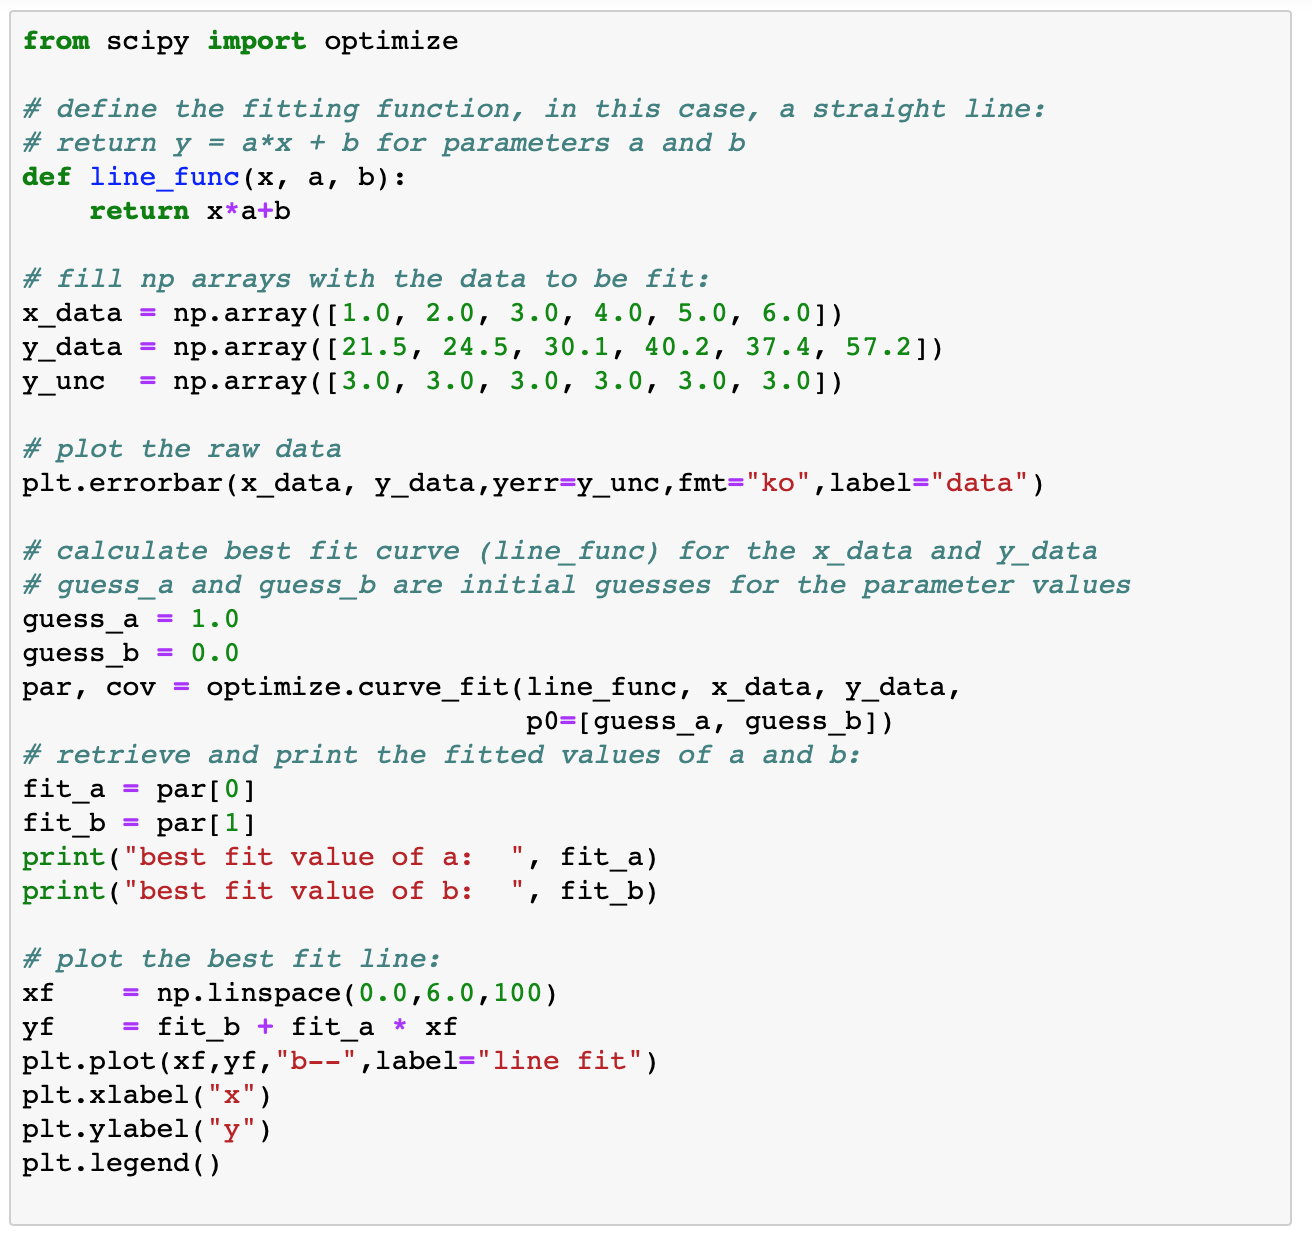
\includegraphics[width=0.65\textwidth]{figs/labs/fitting/fit_code.png} \\
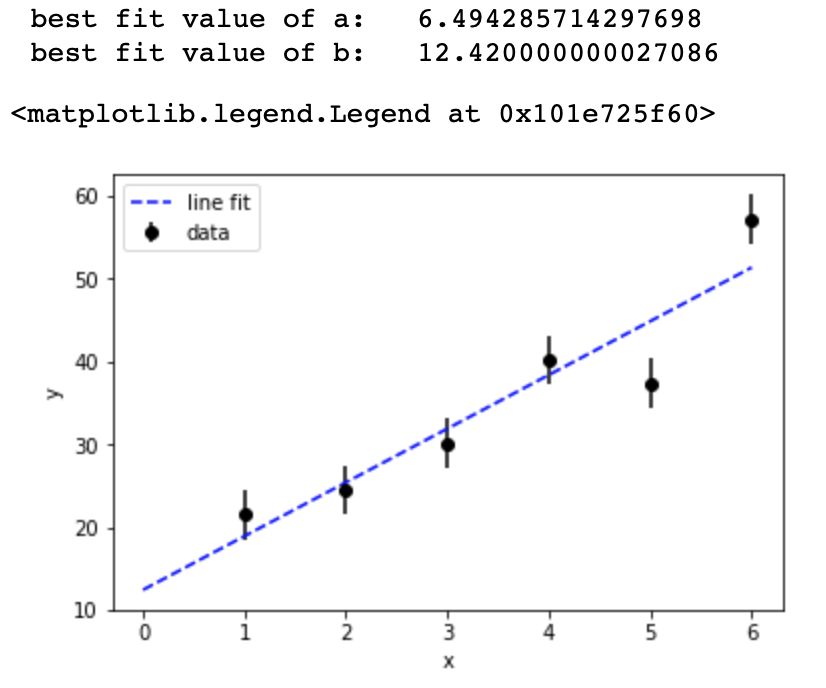
\includegraphics[width=0.65\textwidth]{figs/labs/fitting/fit_out.png} \\
\caption{Example fitting data to straight line.}
\label{fig:fiteg}
\end{center}
\end{figure}

An example using Scientific Pythons {\tt curve{\_}fit} function to fit
a straight line to data is shown in Fig.~\ref{fig:fiteg}.  A block of 
code defining the function we wish to fit, in this case, a straight
line, is defined as a function:
\begin{verbatim}
     def line_func(x, a, b):
         return a*x + b
\end{verbatim}
In this case, the function requires three parameters (in the computer
science sense, not the mathematical sense) the x data in a numpy array
as function parameter x, the slope as function parameter a, and the
intercept as function parameter b.  When called, the function returns
the x data multiplied by the value a, with the value b added.  We
don't directly call this function, but in principle, it could be
called like:
\begin{verbatim}
    y_data = line_func(x_data, 2.0, 0.0)
\end{verbatim}
to create a numpy array {\tt y{\_}data} constructed from {\tt
  x{\_}data} with slope 2 and intercept 0.

The next section filling numpy arrays containing the data, and
plotting it with error bars should be familiar by now.  The fit itself
is performed by the line:
\begin{verbatim}
par, cov = optimize.curve_fit(line_func, x_data, y_data, p0=[guess_a, guess_b])
\end{verbatim}
This performs a fit of the function {\tt line{\_}func} defined above
to the $x$ and $y$ data contained in the arrays {\tt x{\_}data} and
{\tt y{\_}data}.  Numerical fits generally find the local minimum,
which is not necessarily the global minimum of interest.  It is
important therefore, especially for complicated fits, to provide an
initial guess near the expected fit values.  These are provided to the
optional, named, function parameter {\tt p0}, which is set to the
python list {\tt [guess{\_}a, guess{\_}b]} which contains our initial guesses for
the fit parameters $a$ and $b$.  The function performs a least-squares
fit to find the best values of $a$ and $b$ which are returned as the
numpy array {\tt par}.  The function also returns the covariance
matrix as the numpy array {\tt cov}.

The remaining code simply uses the best fit values to plot the fitted
function as a dashed line.  Numerical fits are fickle.  Even if you
are only interested in the fitted value, you should always plot the
best-fit function and compare the results to your data as in important
check for your work.

\begin{table}
\caption{Sample data for straight line fit.}
\label{tbl:linesamp}
\begin{center}
\begin{tabular}{ll}
$x$ & $y \pm \sigma_y$ \\
1.0  & $15.9 \pm 3.0$ \\
2.0  & $23.6 \pm 3.0$ \\
3.0  & $33.9 \pm 3.0$ \\
4.0  & $39.7 \pm 3.0$ \\
5.0  & $45.0 \pm 10.0$ \\
6.0  & $32.4 \pm 20.0$ \\
\end{tabular}
\end{center}
\end{table}

\begin{figure}[htbp]
\begin{center}
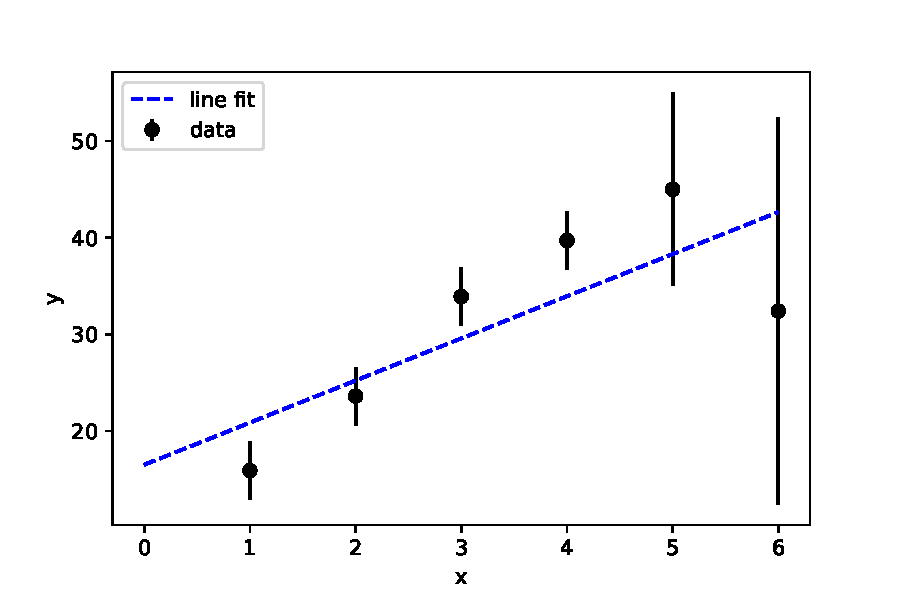
\includegraphics[width=0.65\textwidth]{figs/labs/fitting/bias.pdf} 
\caption{This linear fit is biased by the failure to properly account for uncertainties.  An unbiased fit would track the well constrained points more closely.}
\label{fig:fitbias}
\end{center}
\end{figure}

\begin{plot}
Apply code like that of Fig.~\ref{fig:fiteg} to the data in
Table~\ref{tbl:linesamp}. Plot the data including error bars and the
best-fit function to obtain a result like that of Fig.~\ref{fig:fitbias}.
\end{plot}

Notice that the last two data points in Table~\ref{tbl:linesamp} have
larger uncertainties than the other data points.  However, the call to
the {curve{\_}fit} function does not provide the parameter
uncertainties, and so the function assumes that they all have the
value $1$.  In this case, since the uncertainties are not in fact all
the same, the function does not find the correct minimum.  The answer
is clearly biased (as in Fig.~\ref{fig:fitbias}) toward the poorly
measured points, because the function gives these points the same
weight as all of the other points.

\begin{plot}
Look-up the {\tt curve{\_}fit} function and the optional parameter
{\tt sigma}. Provide the correct uncertainties to the fit and make a
new plot with the data and the fit.  You should observe that the fit
results is no longer biased, and more closely tracks the well
constrained left side of the plot.
\end{plot}

\section{Parameter Uncertainties}

\begin{figure}[htbp]
\begin{center}
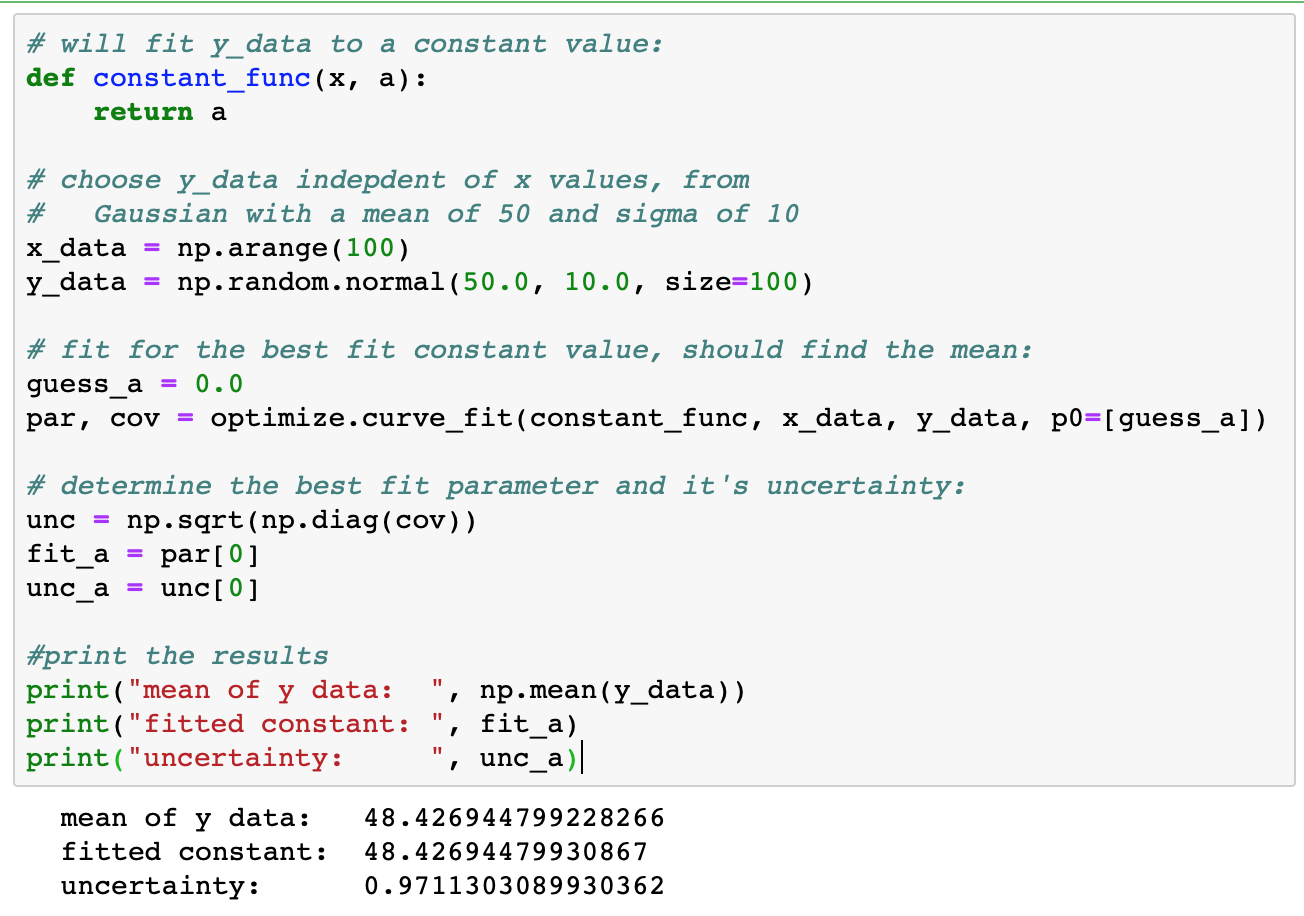
\includegraphics[width=0.65\textwidth]{figs/labs/fitting/uncertainties.png} \\
\caption{Example obtaining parameter uncertainties.}
\label{fig:fitunc}
\end{center}
\end{figure}

We will show in lecture that the uncertainty $\sigma_{p_i}$ on the $i$th parameter $p_i$
can be determined from the second derivative of the $\chi^2$ function:
\begin{displaymath}
\frac{d^2\chi^2}{d p_i^2} = \frac{2}{\sigma_{p_i}^2}.
\end{displaymath}
In general, for $M$ parameters, the $M \times M$ covariance matrix is calculated as:
\begin{displaymath}
C(i,j) = 2 \cdot \left(\dfrac{d^2\chi^2}{d p_i d p_j} \right)^{-1}
\end{displaymath}
from which we can see that the diagonals are simply the parameter uncertainties squared:
\begin{displaymath}
C(i,i) = 2 \cdot \left(\dfrac{d^2\chi^2}{d p_i^2} \right)^{-1} = \sigma^2_{p_i}.
\end{displaymath}
The off-diagonal elements contain information about how parameters are
correlated, and for a well designed fit function they should be close to
zero.

The {\tt curve{\_}fit} function returns both the best fit parameter values and the covariance matrix:
\begin{verbatim}
par, cov = optimize.curve_fit(...)
\end{verbatim}
For a fit with $M$ parameters, we can obtain an array containing the
$M$ parameter uncertainties from the square root of the diagonals of the $M \times M$
covariance matrix:
\begin{verbatim}
unc = np.sqrt(np.diag(cov))
\end{verbatim}

An example is shown in Fig.~\ref{fig:fitunc}, for a single parameter.
In this case, the $y$-values are simply 100 random numbers drawn from
a Gaussian distribution with mean $m = 50$ and a width $\sigma_y =10$.
The best fit constant value is simply the mean of the $y$-values.  The
uncertainty on the mean value should be:
\begin{displaymath}
\sigma_m = \sigma_y / \sqrt{N} = 10 / \sqrt{100} = 1.0
\end{displaymath}
Indeed we obtain a best fit constant value and it's uncertainty close
to these expected values.

It's surprising actually, that the fit returns the correct
uncertainty.  Look through the code carefully and notice that nowhere
has the uncertainty on the $y$ parameters $\sigma_y$ been provided to
the fit.  So how can it possibly deduce the correct uncertainty
$\sigma_m = \sigma_y / \sqrt{N}$?

The answer is that behind the scenes, the {\tt curve{\_}fit} function
is being really quite clever (too clever, in my opinion, for a default
behavior!)  By default, the covariance matrix returned by the 
{\tt curve{\_}fit} function is scaled by the factor:
\begin{displaymath}
\alpha = \frac{\chi^2_{\rm min}}{\rm NDF}
\end{displaymath}
the minimum value of the $\chi^2$ divided by the number of degrees of
freedom (number of data points minus number of parameters).  We'll
show in lecture that $\alpha$ is around 1 for a least-squares fit with
an appropriate model and correct uncertainties.  So nominally this
factor is one, and has no effect.  But consider what happens if the
actual uncertainties are $\sigma$ while the $\chi^2$ used in the fit assumes they
are, for example, ``1''.  In this case, the calculated $\chi^2$ is:
\begin{displaymath}
\chi^2 = \sum_i \frac{(f(x_i;p) - y_i) ^2}{1}
\end{displaymath}
which differs from the correct $\chi^2$:
\begin{displaymath}
\chi^2 = \sum_i \frac{(f(x_i;p) - y_i) ^2}{\sigma^2}
\end{displaymath}
by a factor of $\sigma^2$.  This means that while the correct value
for $\alpha$ is nearly one, the calculated value of alpha will be
$\sigma^2$.  This is precisely the factor needed to scale the squared
parameter uncertainties to account for the fact that the initial
uncertainty was $\sigma$ but we assumed $1$.

This behavior is controlled by the parameter {\tt absolute{\_}sigma}.
By default, the function sets {\tt absolute{\_}sigma = False} and
scales the covariance matrix as just described.  On the other hand, if
you want to simply use the provided uncertainties without re-scaling
the covariance matrix, you must remember to set {\tt
  absolute{\_}sigma=False}.  I think this is a really poor choice of
default behavior...  it's really quite a fancy thing to do implicitly.
In cases when you know the uncertainty on your data points, this
re-scaling actually results in less correct estimate for the
uncertainties.  This is because for a good model with proper
uncertainties, the factor $\alpha$ is near one, but not exactly one.



\begin{plot}
Repeat the fit in Fig.~\ref{fig:fitunc}, but
set the uncertainties on the $y$ values to 10 and also set 
{\tt absolute{\_}sigma = True} in the fit.  Record the uncertainty.
\end{plot}

\begin{plot}
Leave the uncertainties on the $y$ values
unspecified and set {\tt absolute{\_}sigma = True} in the fit.  You
should obtain an uncertainty of $0.1$.  Record your value and explain
why you obtained this value.
\end{plot}

As a rule of thumb, when using {\tt curve{\_}fit}, if you provide
explicit uncertainties, you should remember to set {\tt
  absolute{\_}sigma=True}.  And really, for precision work, you should
almost always be providing explicit uncertainties.

\section{Fitting a Sine Curve}

In this section, you will fit the sample data to a sine function:
\begin{displaymath}
 y = A \, \sin( k x). 
\end{displaymath}
Use the following sample data:\\
\begin{center}
\begin{tabular}{|ll| ll|ll|}
\hline
$x$ & $y$ & $x$ & $y$ & $x$ & $y$\\
\hline
0  & 5.3    & 4  & -9.7   & 8  & 15.7  \\
1  & 15.0   & 5  & -17.4  & 9  & 18.5  \\
2  & 19.2   & 6  & -20.5  & 10 & 8.6   \\
3  & 6.8    & 7  &  2.1   & &  \\
\hline
\end{tabular}
\end{center}
Assume the uncertainty is the same for each $y$ value: $\sigma_i = 2$.

\begin{plot}
Plot the sample data including error bars and the best-fit sine wave.  Print
the best fit parameter values and their uncertainties.  This fit is
highly sensitive to the initial guess, so make sure you provide good
starting values close the correct answer.  Remember to set {\tt
  absolute{\_}sigma=True}.
\end{plot}


